\documentclass{article}
\usepackage[utf8]{inputenc}

\title{KREPE Flight Computer Software and Safety Verification}
\author{Matt Ruffner}
\date{March 2020}

\usepackage{url}
\usepackage{float}
\usepackage{natbib}
\usepackage{graphicx}
\usepackage{listings}
\usepackage{fullpage}
\usepackage{hyperref}
\hypersetup{
    colorlinks=true,
    linkcolor=blue,
    filecolor=magenta,      
    urlcolor=cyan,
}

\begin{document}

\maketitle

\section{General Requirements Compliance}
Upon both power up (after primary activation via pull-tab) and detection of a termination or off-nominal power condition, the Teensy processor will enter a safe reset state, where all GPIO pins controlling critical system functions are set to a high impedance value. This high impedance state, in addition to the flight computer PCB, ensure requirements in the \textit{General Requirements for the Computer-Based Control System Safety Requirements for the ISS} are met. Overcurrent and undervoltage protection for battery cells is implemented upstream of the flight computer, limiting the off-nominal power conditions expected (see KREPE Flight Computer Hardware Manual). See Fig. \ref{fig:exec-lifecycle} for an overview of the main execution lifecycle and how upon both power up and detection of an abnormal power condition both put the CBCS back into the safe high impedance state. CBCS General Requirements are discussed below.

\subsection{Req. 3.1.1.1}
Teensy 3.5 controller documentation shows that the controller powers up into the known safe reset state. No outputs occur until the processing state is initiated (see Fig. \ref{fig:exec-lifecycle}). Verification for this requirement will monitor the state of Teensy output pins with external hardware upon power up to make sure specific signals (i.e. iridium soli state relay activation signal) do not transition unexpectedly. 

\subsection{Req. 3.1.1.2}
KREPE flight computer software on the Teensy 3.5 controller enters a safe state in the event that a termination condition is detected (e.g. low system battery  voltage; see Fig. \ref{fig:exec-lifecycle}). As the KREPE capsule is incapable of receiving any external commands, the detection of a termination command scenario is not applicable. Testing for compliance with this requirement entails monitoring of Flight computer pin state with external hardware while the system experiences low battery voltage to make sure it places critical pins in a high impedance or off state.

\subsection{Req. 3.1.1.3}
The KREPE battery protection subsystem prevents any overcurrent or undervoltage conditions from reaching the flight computer. The main off-nominal power condition the flight computer may encounter is power failure. The Teensy 3.5 controller features a power management controller that will place it in a safe reset state if a power failure is detected. The KREPE flight computer also  monitors system battery voltage to preemtively detect an off-nominal power condition and place the system in the safe state (see Fig. \ref{fig:exec-lifecycle}).

\begin{figure}
  \centering
  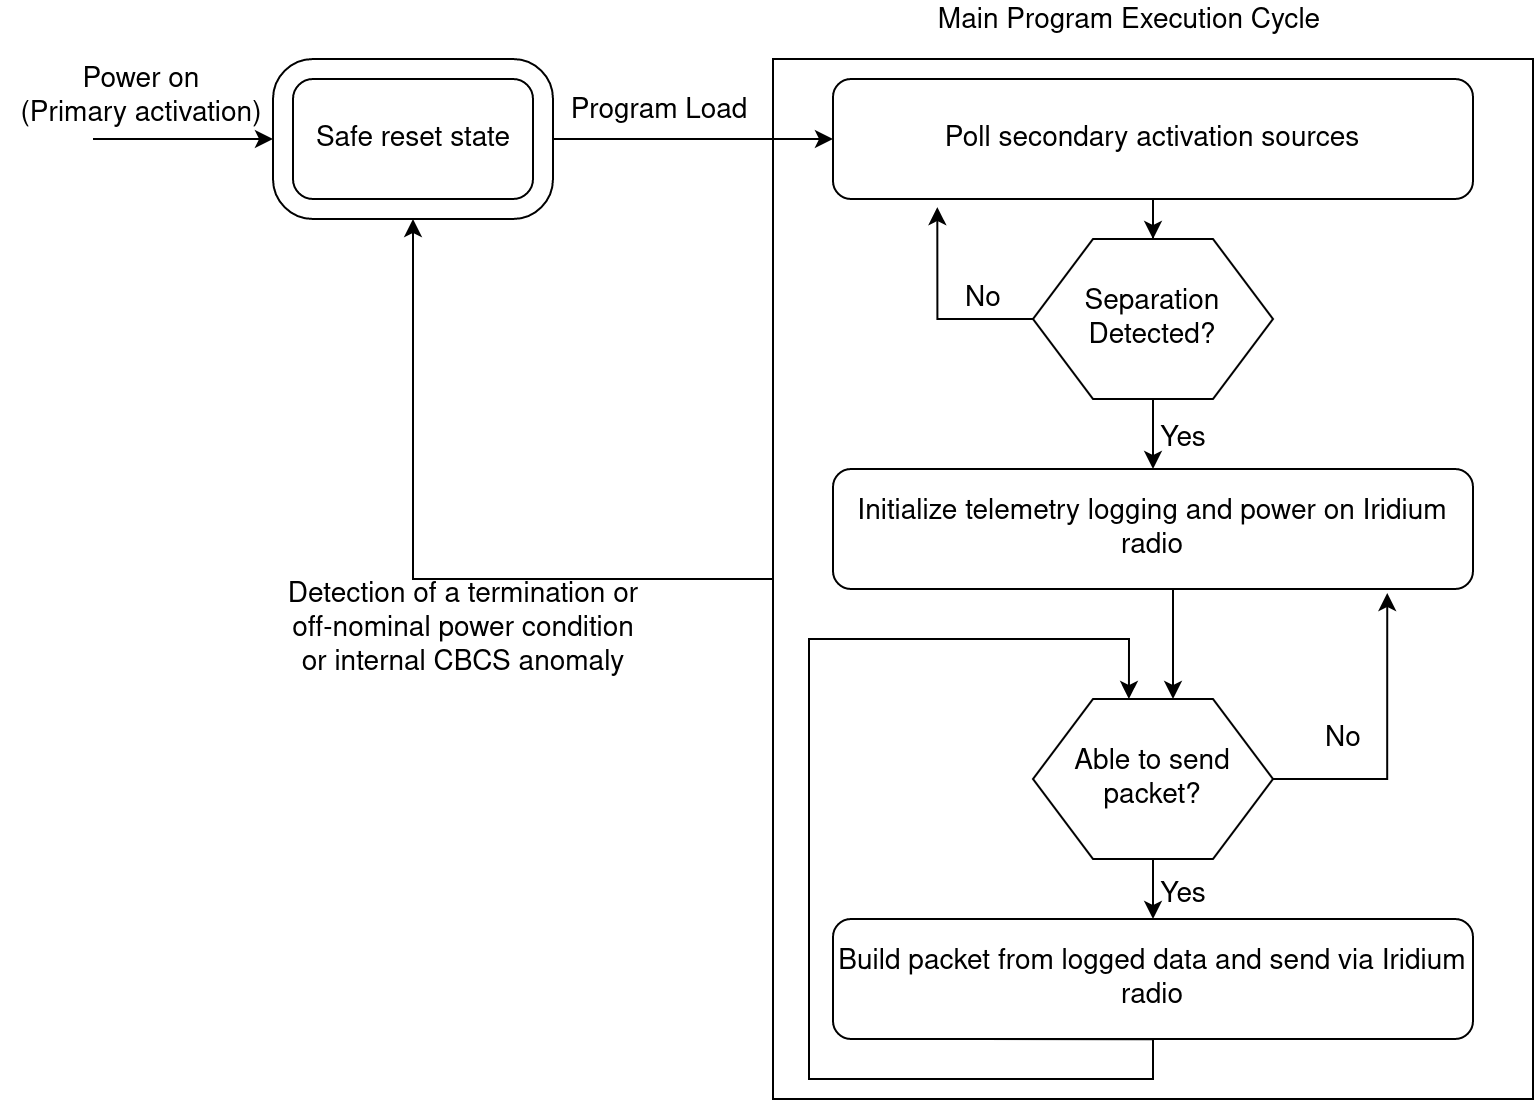
\includegraphics[width=0.75\textwidth]{images/software-overview.png}
  \caption{Overview of main execution cycle showing return to safe high-Z reset state upon startup and abnormal power condition.}
  \label{fig:exec-lifecycle}
\end{figure}

\subsection{3.1.1.4}
N/A

\subsection{3.1.1.5}
N/A

\subsection{3.1.1.6}
The metal enclosure that houses the KREPE module acts as a Faraday cage and mitigates the risk imposed to the CBCS by inadvertent memory modification.

\subsection{3.1.1.7}
Upon detection of an anomaly internal to the CBCS there is watchdog timer functionality that will return the CBCS to the known safe initialization state. Verification procedures for this requirement entail physical disruption/disconnection of flight computer hardware to ensure control software can recover.

\subsection{3.1.1.8}
The external sources in this case would be the ambient temperature of capsule and the presence of the metal enclosure around the KREPE capsule. The capsule uses the Fault flags on the thermocouple to digital converter are used to discern if a valid thermocouple reading has been collected or not. There are also multiple thermocouples whos values are cross checked for consistency in valid readings. Capacitive sensing is also used to detect the presence of the metal enclosure around the KREPE capsule. Both of these inputs are used to discern between valid and invalid input.

Verification for this requirement entails physical disconnection/perturbation of thermocouple and capacitive sensing leads to analyze the induced effect on measurement values and fault conditions. 

\subsection{3.1.1.9}
See Fig. \ref{fig:exec-lifecycle} for KREPE software design requirements.

\subsection{3.1.1.10}
Full system software is available upon request.

\subsection{3.1.1.11}
No external data or command transmissions are made prior to activation of Iridium radio. We stay dormant until secondary activation, this req looks like it applies to much more sophisticated craft. The KREPE capsule is a highly integrated device comprised of only one flight computer PCB and radio module. Integrity checks are preformed by the Iridium radio module to verify a correct command was sent. Prior to secondary activation, integrity checks are also performed on readings from secondary activation decision sources (thermocouples) to ensure errant reading do not trigger an activation (see Req. 3.1.1.8).

\subsection{3.1.1.12}
N/A

\subsection{3.1.1.13}
N/A




%%%%%%%%%%%%%%%%%%%%%%%%%%%%%%%%%%%%%%%%%%%%%%%%%%%%%%%%%%%%%%%%%%%%%%%%%%%%%%%%%%%
%%%%%%%%%%%%%%%%%%%%%%%%%%%%%%%%%%%%%%%%%%%%%%%%%%%%%%%%%%%%%%%%%%%%%%%%%%%%%%%%%%%
%%%%%%%%%%%%%%%%%%%%%%%%%%%%%%%%  APPENDIX
%%%%%%%%%%%%%%%%%%%%%%%%%%%%%%%%%%%%%%%%%%%%%%%%%%%%%%%%%%%%%%%%%%%%%%%%%%%%%%%%%%%
%%%%%%%%%%%%%%%%%%%%%%%%%%%%%%%%%%%%%%%%%%%%%%%%%%%%%%%%%%%%%%%%%%%%%%%%%%%%%%%%%%%
%\appendix

%\newpage
%\section{Arduino Pin Mapping}
%\label{app:pinmap}
%\lstinputlisting[language={}]{arduino-pinmap.txt}

%\bibliographystyle{plain}
%\bibliography{references}
\end{document}
